% Chapter 2: Physics and Computation

Three people walk into a room with the same problem. A logistics manager needs
the shortest route through a hundred cities. A physicist needs the lowest
energy state of a hundred interacting spins. A computer scientist needs to
prove that no algorithm can find the answer faster than brute search. They are
all navigating the same exponentially large space of configurations, and they
will all get stuck in the same ways. But they will formalize the problem
differently, and that difference will determine what each of them can prove.

This chapter builds the vocabulary that makes that claim precise. The path runs
from physics through complexity theory to the adiabatic mechanism, and each
piece earns its place by answering a question the previous piece leaves open.

\section{Reality}
\label{sec:ch2-reality}

What does it mean to choose a formalization? It means committing to which
aspects of physical reality the mathematics captures. This thesis needs one
such commitment: mathematics models regularities in the physical world but
does not replace the world itself.

The consequence is immediate. A complexity claim is meaningful only after the
computational model and the resource accounting are fixed. If access to the
input changes, if precision demands change, or if the available control
primitives change, the same task can move from easy to hard. Hardness is not an
intrinsic property of a problem. It is a joint property of the problem, the
model, and the resources being counted.

A concrete example makes this vivid. Finding the minimum of a function
$f:\{0,1\}^n\to\mathbb{R}$ with no promise about its structure requires
checking nearly every input in the worst case. In a classical query model this
costs $\Theta(2^n)$ evaluations. In a quantum query model the same task costs
$\Theta(2^{n/2})$ evaluations \cite{Grover1996, bennett1997strengths}. The
function did not change. The counting of resources did not change. Only the
model of computation changed, and with it the sharp boundary between efficient
and inefficient.

The dependence on model choice will recur throughout this thesis, and it helps
to have a picture for it.
\begin{figure}[h]
\centering
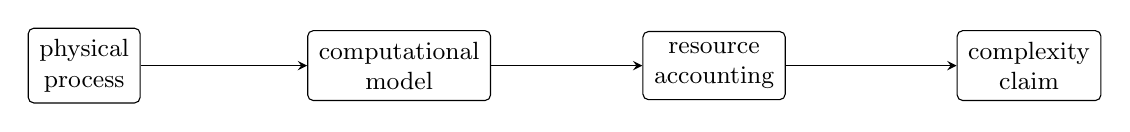
\begin{tikzpicture}[
  box/.style={draw, rounded corners=2pt, align=center, inner sep=4pt, font=\small},
  arr/.style={->, >=stealth, line width=0.5pt}
]
\node[box] (p) at (0,0) {physical\\process};
\node[box] (m) at (4.0,0) {computational\\model};
\node[box] (r) at (8.0,0) {resource\\accounting};
\node[box] (c) at (12.0,0) {complexity\\claim};
\draw[arr] (p) -- (m);
\draw[arr] (m) -- (r);
\draw[arr] (r) -- (c);
\end{tikzpicture}
\caption{The modeling chain: physical assumptions determine the computational
model, which determines resource accounting, which supports or refutes
complexity claims.}
\label{fig:ch2-modeling-chain}
\end{figure}
Physical assumptions determine a computational model. The model determines a
resource accounting. And the resource accounting supports, or fails to support,
a complexity claim. Chapters~3 and~4 will put this chain under pressure: the
optimization objective stays fixed while the computational model shifts from
query circuits to continuous Hamiltonian evolution.

\section{Physics}
\label{sec:ch2-physics}

The modeling chain begins with physics, and physics contributes a single object
that will persist through every chapter of this thesis: the Hamiltonian. Energy
plays a double role. It generates the dynamics of a system, and it
simultaneously defines what it means for a configuration to be preferred. This
double role is what connects physics to optimization.

In classical mechanics, a system with $f$ degrees of freedom lives in a phase
space of generalized coordinates $q_1,\ldots,q_f$ and conjugate momenta
$p_1,\ldots,p_f$. The Hamiltonian $H_{\mathrm{cl}}(q,p)$ determines the full
time evolution through Hamilton's equations
\begin{equation}
\label{eq:ch2-hamilton-equations}
\dot{q}_j = \frac{\partial H_{\mathrm{cl}}}{\partial p_j},
\qquad
\dot{p}_j = -\frac{\partial H_{\mathrm{cl}}}{\partial q_j}.
\end{equation}
The rate of change of each variable is set by how the energy depends on its
conjugate. The Hamiltonian does not merely label states by their energy. It
generates the flow that carries one state to the next.

Statistical mechanics introduces the second role. When a system is coupled to a
heat bath at temperature $T$, the probability of finding it in configuration
$z$ is not uniform. Low-energy configurations are exponentially preferred. For
a cost profile $C(z)$ and inverse temperature $\beta = 1/(k_B T)$, the Gibbs
distribution assigns probabilities
\begin{equation}
\label{eq:ch2-gibbs}
\pi_\beta(z)=\frac{e^{-\beta C(z)}}{Z_\beta},
\qquad
Z_\beta=\sum_z e^{-\beta C(z)}.
\end{equation}
As $\beta\to\infty$, mass concentrates on the minimizers of $C$. The mechanism
is direct: for any non-optimal configuration $z$, the ratio
$\pi_\beta(z)/\pi_\beta(z^*)=e^{-\beta(C(z)-C_{\min})}$ vanishes
exponentially as $\beta$ grows. Finding the ground state is what thermal
equilibrium does at zero temperature. The partition function $Z_\beta$ encodes
the full thermodynamic content of the system, and evaluating it turns out to
be, in general, computationally hard. Section~\ref{sec:ch2-sharpp} will make
that precise.

Quantum mechanics preserves the Hamiltonian as generator but changes the arena.
The state is now a unit vector $\ket{\psi}$ in a Hilbert space, the
Hamiltonian is a Hermitian operator, and with $\hbar=1$ the evolution law is
\begin{equation}
\label{eq:ch2-schrodinger-linear}
i\frac{d}{dt}\ket{\psi(t)}=H(t)\ket{\psi(t)}.
\end{equation}
The ground state of $H$ is its minimum-energy eigenstate, and finding it is
the quantum analogue of minimizing a cost function. The eigenvalue structure of
the Hamiltonian, specifically the spectral gap between the ground state and the
first excited state, will turn out to control how long an adiabatic algorithm
must run. Sections~\ref{sec:ch2-spectral-complexity}
and~\ref{sec:ch2-adiabaticity} develop this connection.

\section{Computation}
\label{sec:ch2-computation}

The spectral gap determines how long the adiabatic algorithm runs. But ``long''
needs a yardstick, and that yardstick comes from complexity theory: a precise
framework for measuring hardness across computational models. Without it,
saying that an adiabatic algorithm is fast or slow would be meaningless.

The baseline model is the Turing machine \cite{arora2009computational}. A
language $L\subseteq\{0,1\}^*$ is decidable if some Turing machine halts on
every input and accepts exactly the strings in $L$. Decidability separates what
can be computed from what cannot. The Church--Turing thesis asserts that every
physically realizable computation can be performed by a Turing machine. The
extended Church--Turing thesis goes further, adding an efficiency claim: every
physically realizable computation can be simulated by a probabilistic classical
machine with at most polynomial overhead \cite{arora2009computational}. Quantum
computation challenges this efficiency claim while leaving computability
untouched \cite{Deutsch1985, BernsteinVazirani1997}. Whether the challenge succeeds is the question this thesis addresses
in the setting of unstructured optimization.

With the model fixed, ``efficient'' means polynomial time.

\begin{definition}[Class $\mathrm{P}$]
A decision problem is in $\mathrm{P}$ if a deterministic Turing machine solves
it in time polynomial in input length.
\end{definition}

Evaluating a cost function $C(z)$ at a given $z$ is typically in $\mathrm{P}$:
substitute values and compute. But minimizing $C$ over all of $\{0,1\}^n$
appears to require searching an exponentially large space. Boolean
satisfiability makes the difficulty concrete. A 3-SAT formula has the form
\begin{equation}
\label{eq:ch2-3sat}
F(x_1,\ldots,x_n)=\bigwedge_{j=1}^{m}(\ell_{j,1}\lor\ell_{j,2}\lor\ell_{j,3}),
\end{equation}
with each literal $\ell_{j,k}$ being either $x_i$ or $\overline{x}_i$. Given a
candidate assignment $x$, checking whether $F(x)=1$ takes time linear in the
formula: evaluate each clause and confirm all are satisfied. A first-year
student can verify a solution. But finding a satisfying assignment from scratch,
or proving that none exists, appears to require effort that grows exponentially
with $n$. This asymmetry between finding and checking is not an accident of
3-SAT. It is the heart of the $\mathrm{P}$ versus $\mathrm{NP}$ question.

\begin{definition}[Class $\mathrm{NP}$]
A decision problem is in $\mathrm{NP}$ if every yes-instance has a certificate
of length polynomial in the input that can be verified in polynomial time by a
deterministic Turing machine.
\end{definition}

Every problem in $\mathrm{P}$ is also in $\mathrm{NP}$, since an efficient
algorithm can serve as its own verifier. The converse, whether
$\mathrm{P}=\mathrm{NP}$, is the most famous open problem in theoretical
computer science. The strong consensus is that $\mathrm{P}\neq\mathrm{NP}$,
but this remains unproved after more than fifty years.

What makes 3-SAT remarkable is not just that it appears hard, but that it
captures the full difficulty of $\mathrm{NP}$. Cook proved that every
efficiently verifiable problem can be translated into an instance of SAT
through a polynomial-time computable function that preserves yes and no answers
\cite{cook1971complexity}. Such a function is called a reduction: it converts
one problem into another while preserving the answer.

\begin{definition}[Polynomial-time many-one reduction]
For decision problems $A$ and $B$, write $A\leq_p B$ if there exists a
polynomial-time computable function $r$ such that
\begin{equation}
\label{eq:ch2-reduction}
x\in A \iff r(x)\in B.
\end{equation}
\end{definition}

A reduction from $A$ to $B$ means that $B$ is at least as hard as $A$: any
algorithm for $B$ immediately yields one for $A$ by composing with $r$, so
hardness flows upward through a hierarchy of problems. A problem to which all
of $\mathrm{NP}$ reduces is NP-hard; if it also lies in $\mathrm{NP}$, it is
NP-complete. Cook proved that SAT is NP-complete; Karp then showed that many
combinatorial problems, including 3-SAT, are NP-complete through polynomial
reductions \cite{Karp1972}. Solving any one of them in polynomial time would
collapse the entire class. The hardness reductions in Chapter~8 of this thesis
begin from exactly this problem.

The point of contact with optimization is threshold decision. Given a cost
function $C$ and a threshold $\tau$, ask whether there exists $z$ with
$C(z)\leq\tau$. For 3-SAT, this asks whether the minimum number of violated
clauses is at most $\tau$. If this threshold language is NP-hard, no generic
polynomial-time algorithm can minimize $C$ over all instances, unless
$\mathrm{P}=\mathrm{NP}$. The adiabatic algorithm's task is precisely this
minimization. The complexity classes just defined measure how hard that task is.

\section{The \texorpdfstring{$\#\mathrm{P}$}{\#P} Complexity Class}
\label{sec:ch2-sharpp}

There is a subtlety the decision framework misses. The spectral parameters that
control adiabatic runtime in Chapters~5 through~8 depend on the degeneracies
$\{d_k\}$ and energy gaps $\{E_k-E_0\}$ of the problem Hamiltonian. Computing
these parameters to the precision the algorithm requires can be
$\#\mathrm{P}$-hard (Chapter~8). The issue is not just whether a solution
exists, but how many solutions exist. For the spectral quantities that govern
this thesis, counting is the operative difficulty.

Two Boolean formulas might both be satisfiable, but one could have a single
satisfying assignment while the other has exponentially many. A decision
algorithm cannot distinguish the two cases. A counting algorithm must, and
counting turns out to be a fundamentally harder task.

\begin{definition}[Class $\#\mathrm{P}$]
A function $f:\{0,1\}^*\to\mathbb{N}$ is in $\#\mathrm{P}$ if there exists a
nondeterministic polynomial-time Turing machine $M$ such that $f(x)$ equals the
number of accepting branches of $M$ on input $x$.
\end{definition}

Valiant introduced $\#\mathrm{P}$ and established the hardness of canonical
counting problems \cite{valiant1979complexity}. The standard example is
\begin{equation}
\label{eq:ch2-sharpsat}
\#\mathrm{SAT}(F)=\left|\left\{x\in\{0,1\}^n : F(x)=1\right\}\right|.
\end{equation}
Decision SAT asks whether this count is nonzero. But computing the exact count
is far harder. $\#\mathrm{P}$ is at least as hard as every class in the
polynomial hierarchy \cite{toda1991pp, arora2009computational}, placing counting strictly
above NP-hard decision problems in a strong structural sense. The permanent of
a $0$-$1$ matrix provides a vivid example: computing it is
$\#\mathrm{P}$-complete \cite{valiant1979complexity}, yet the closely related
determinant is computable in polynomial time. A single sign change in the
summation separates efficient computation from intractability.

The ground-state degeneracy $d_0=|\{z:C(z)=C_{\min}\}|$ is exactly such a
counting object. Adiabatic runtime depends on the full degeneracy spectrum
through spectral parameters defined in Chapter~5. Chapter~8 proves that
approximating the key parameter $A_1$ to additive precision
$\varepsilon<1/(72(n-1))$ is NP-hard. The $\#\mathrm{P}$-hardness result is
stronger: $O(\mathrm{poly}(n))$ exact oracle queries to the spectral parameter
suffice to extract the degeneracy $d_0$ by polynomial interpolation, and
computing $d_0$ is $\#\mathrm{P}$-hard. Near-exact estimation at precision
$\varepsilon\in O(2^{-\mathrm{poly}(n)})$ therefore inherits
$\#\mathrm{P}$-hardness \cite{braida2024unstructured}.

\section{Spectral Complexity}
\label{sec:ch2-spectral-complexity}

Where does counting complexity meet quantum dynamics? In the eigenvalue
structure of the Hamiltonian. The Schr\"{o}dinger
equation~\eqref{eq:ch2-schrodinger-linear} is linear in the state vector,
without approximation. For a time-independent Hamiltonian it has the explicit
solution $\ket{\psi(t)}=e^{-iHt}\ket{\psi(0)}$, and even for time-dependent
Hamiltonians the evolution remains a linear map on $\mathcal{H}$. One might
expect that linearity implies computational simplicity. It does not.

The difficulty resides not in the evolution equation but in the spectrum.
Consider an interpolation $H(s)=(1-s)H_0+sH_z$ between an initial Hamiltonian
$H_0$ (whose ground state is easy to prepare; Chapter~4 specifies the concrete
choice) and a problem Hamiltonian $H_z$ diagonal in the computational basis,
with $s$ ranging from $0$ to $1$. As $s$ varies, the eigenvalues of $H(s)$
trace curves. When two of these curves approach each other, they generically do
not cross. Instead they undergo an avoided crossing: the curves repel, reaching
a minimum separation before diverging again
(Figure~\ref{fig:ch2-avoided-crossing}). The width of this avoided crossing
and the value of $s$ at which it occurs depend on the global structure of both
Hamiltonians. For an $n$-qubit problem Hamiltonian with up to $2^n$
eigenvalues, the crossing geometry is determined by the full set of energies
and degeneracies.

\begin{figure}[h]
\centering
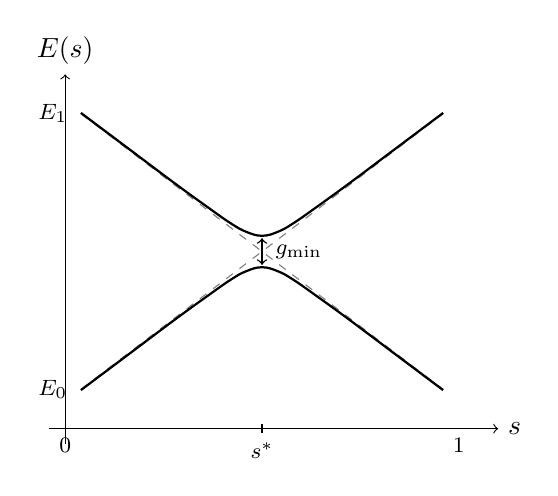
\begin{tikzpicture}
  \draw[->, line width=0.4pt] (-0.2,0) -- (5.5,0) node[right] {$s$};
  \draw[->, line width=0.4pt] (0,-0.2) -- (0,4.5) node[above] {$E(s)$};
  \node[below] at (0,0) {\footnotesize $0$};
  \node[below] at (5,0) {\footnotesize $1$};
  \draw (2.5,0.06) -- (2.5,-0.06);
  \node[below] at (2.5,-0.06) {\footnotesize $s^*$};
  \draw[dashed, gray] (0.2,0.5) -- (4.8,4.0);
  \draw[dashed, gray] (0.2,4.0) -- (4.8,0.5);
  \draw[thick] plot[smooth, tension=0.7] coordinates {
    (0.2,0.49) (0.8,0.94) (1.4,1.39) (1.8,1.68) (2.1,1.89)
    (2.3,2.00) (2.5,2.05) (2.7,2.00) (2.9,1.89) (3.2,1.68)
    (3.6,1.39) (4.2,0.94) (4.8,0.49)
  };
  \draw[thick] plot[smooth, tension=0.7] coordinates {
    (0.2,4.01) (0.8,3.56) (1.4,3.11) (1.8,2.82) (2.1,2.61)
    (2.3,2.50) (2.5,2.45) (2.7,2.50) (2.9,2.61) (3.2,2.82)
    (3.6,3.11) (4.2,3.56) (4.8,4.01)
  };
  \draw[<->, line width=0.5pt] (2.5,2.08) -- (2.5,2.42);
  \node[right, font=\footnotesize] at (2.55,2.25) {$g_{\min}$};
  \node[left, font=\footnotesize] at (0.15,0.5) {$E_0$};
  \node[left, font=\footnotesize] at (0.15,4.0) {$E_1$};
\end{tikzpicture}
\caption{Avoided crossing in the spectrum of $H(s)=(1-s)H_0+sH_z$. Dashed
lines show the eigenvalues that would result if the two Hamiltonians did not
couple; they cross at $s=s^*$. Solid curves show the actual eigenvalues, which
repel near the would-be crossing. The minimum gap $g_{\min}$ sets the internal
timescale of the quantum system:
Section~\ref{sec:ch2-adiabaticity} makes precise how it controls runtime.}
\label{fig:ch2-avoided-crossing}
\end{figure}

This is where computational hardness enters. Small perturbations to a
Hamiltonian can rearrange its eigenvalue structure entirely: spectral gaps can
close exponentially, avoided crossings can narrow or widen, degenerate
subspaces can split. These spectral rearrangements control algorithmic runtime,
and predicting them is NP-hard in general (Chapter~8). The interpolation
between two Hamiltonians can be written in a single line. The location and
width of the avoided crossing that controls the adiabatic algorithm's runtime
depends on the full eigenvalue structure of the problem Hamiltonian, a
structure that can itself be computationally hard to characterize. The
evolution is simple. The geometry it must navigate is not.

\section{Optimization}
\label{sec:ch2-optimization}

How does a combinatorial cost function become an energy spectrum? The
translation is exact, requires no relaxation or rounding, and preserves every
feature that makes the problem hard.

Write the optimization objective as
\begin{equation}
\label{eq:ch2-cost-min}
\min_{z\in\{0,1\}^n} C(z),
\end{equation}
and define the diagonal Hamiltonian
\begin{equation}
\label{eq:ch2-hz}
H_z=\sum_{z\in\{0,1\}^n} C(z)\ket{z}\bra{z}.
\end{equation}
The ground states of $H_z$ are exactly the minimizers of $C$. The
combinatorial objective has become an energy spectrum, and finding the optimum
has become finding the ground state.

For SAT, the encoding is explicit. Let $\chi_j(x)\in\{0,1\}$ indicate whether
assignment $x$ satisfies clause $j$, and define the penalty function
\begin{equation}
\label{eq:ch2-sat-penalty}
C_F(x)=\sum_{j=1}^m\bigl(1-\chi_j(x)\bigr).
\end{equation}
Then $F$ is satisfiable if and only if $\min_x C_F(x)=0$. Each unsatisfied
clause contributes a unit penalty, so $C_F$ counts the number of violations.

Counting resurfaces at the optimum. If $C_{\min}$ denotes the minimum cost,
the ground-state degeneracy is
\begin{equation}
\label{eq:ch2-d0-count}
d_0=\left|\left\{z\in\{0,1\}^n : C(z)=C_{\min}\right\}\right|.
\end{equation}
Even an algorithm that outputs a single optimizer has runtime that depends,
through the spectral structure of $H_z$, on how many optimizers exist. The
spectral parameters controlling adiabatic runtime (defined in Chapter~5) are
functions of the complete set of degeneracies $\{d_k\}$ and energy gaps
$\{E_k-E_0\}$. A single-solution algorithm cannot escape the influence of a
counting object.

A canonical hard family illustrating the encoding is the Ising model on a
graph $G=(V,E)$
\begin{equation}
\label{eq:ch2-ising}
H_\sigma=\sum_{(i,j)\in E}J_{ij}\sigma_z^i\sigma_z^j+
\sum_{j=1}^{n} h_j\sigma_z^j,
\end{equation}
where $\sigma_z^j$ is the Pauli-$Z$ operator on site $j$ (Chapter~3 develops
the formalism), the first sum runs over edges of $G$ with couplings $J_{ij}$,
and the second sum includes local fields $h_j$. Many NP-hard combinatorial
objectives map directly to this form
\cite{barahona1982computational, lucas2014ising}.
Weighted MaxCut provides a transparent example. For $x_i\in\{0,1\}$, the cut
value is
\begin{equation}
\label{eq:ch2-maxcut}
C_{\mathrm{cut}}(x)=\sum_{(i,j)\in E}w_{ij}(x_i\oplus x_j),
\end{equation}
and under the spin substitution $\sigma_i=(-1)^{x_i}$ this becomes
\begin{equation}
\label{eq:ch2-maxcut-ising}
C_{\mathrm{cut}}(\sigma)=\frac{1}{2}\sum_{(i,j)\in E}w_{ij}(1-\sigma_i \sigma_j).
\end{equation}
The correspondence is $J_{ij}=-w_{ij}/2$ and $h_j=0$: the total weight of
edges crossing the cut is an antiferromagnetic Ising interaction energy. Any
graph optimization objective expressible as pairwise interactions maps to an
Ising model with no auxiliary variables, making the spectral analysis of
Chapter~5 directly applicable. Combinatorial objectives and spin Hamiltonians
are the same mathematical object. The encoding was
introduced in the adiabatic context by Farhi et al.
\cite{farhi2000adiabatic, farhi2001adiabatic}, and it means that any NP-hard
optimization objective can be attacked with Hamiltonian methods. Runtime
analysis then reduces entirely to the spectral analysis of $H_z$, which is the
subject of Sections~\ref{sec:ch2-adiabaticity}
and~\ref{sec:ch2-energy-landscapes}.

\section{Adiabaticity}
\label{sec:ch2-adiabaticity}

The Hamiltonian $H_z$ encodes the cost function. What remains is a mechanism
for finding its ground state without knowing the answer in advance. The
mechanism this thesis studies is adiabatic evolution, and understanding it
requires understanding what ``slow'' means in quantum mechanics.

The word adiabatic comes from the Greek \textit{adiabatos}, meaning
``impassable,'' and entered physics through Clausius for processes with no heat
exchange across system boundaries. The meaning in quantum mechanics differs
from the thermodynamic original, but both rest on a shared structure: two
competing timescales. Every adiabatic process has an external timescale, set by
how rapidly conditions change, and an internal timescale, set by how rapidly
the system can respond. Adiabaticity holds when external change is slow
relative to internal response. In thermodynamics, the internal timescale is the
relaxation time to local equilibrium: compress a gas slowly enough and it
remains in equilibrium throughout. In quantum mechanics, the internal timescale
is the inverse spectral gap. There is no absolute meaning of ``slow.'' Slow is
always slow compared to something.

For a quantum system governed by a time-dependent Hamiltonian $H(t)$, the
internal timescale is set by the energy gap between eigenstates. At each
instant, $H(t)$ has a spectrum of eigenstates and eigenvalues. If the system
begins in an eigenstate and the Hamiltonian changes slowly enough, the state
tracks the instantaneous eigenstate. It remains an eigenstate of $H(t)$ at
every moment, even as the eigenstate itself changes character. If the
Hamiltonian changes too rapidly, the state develops overlap with other
eigenstates and the system has made a transition \cite{BornFock1928, Kato1950}.
In the context of an algorithm, this transition is a failure.

Why does the gap control transitions? The physical mechanism comes from
first-order time-dependent perturbation theory. When the Hamiltonian changes,
the amplitude for transitioning from the instantaneous ground state
$\ket{e_0(t)}$ to an excited state $\ket{e_n(t)}$ acquires a factor
\begin{equation}
\label{eq:ch2-transition-amplitude}
\frac{\bra{e_n(t)}\dot{H}(t)\ket{e_0(t)}}{E_n(t)-E_0(t)}.
\end{equation}
The energy denominator tells the story. Transitions to nearby energy levels are
enhanced while transitions to distant levels are suppressed. The dominant
leakage channel is the nearest excited state, and the gap
$g(t)=E_1(t)-E_0(t)$ sets the relevant scale. The inverse gap $1/g(t)$ is the
internal response timescale: the natural oscillation period between the two
lowest eigenstates. For the Hamiltonian to change negligibly over this period,
the fractional change per oscillation must be small compared to the gap itself.

This reasoning yields the adiabatic heuristic condition
\cite{jansen2007bounds}
\begin{equation}
\label{eq:ch2-adiabatic-heuristic}
\frac{\|\dot{H}(t)\|}{g(t)^2}\ll 1,
\end{equation}
where $\|\cdot\|$ denotes the spectral norm. This is the physical motivation
behind every runtime bound in this thesis. Total evolution time $T$ must be
large enough that the sweep rate $\|\dot{H}(t)\|$ remains small relative to
$g(t)^2$ at every point along the Hamiltonian path, requiring at minimum
$T=\Omega(1/g_{\min}^2)$. The minimum gap along the path is the bottleneck.
Small gaps force slowness, and that forced slowness is the computational cost.
The heuristic captures the right qualitative scaling, but the rigorous version
of the adiabatic theorem \cite{jansen2007bounds, ElgartHagedorn2012} involves
additional terms: the degeneracy of the ground state, norms of higher
derivatives of $H(s)$, and an integral bound rather than a pointwise one.
Chapter~4 states the precise result and derives the runtime from it.

The Landau--Zener formula makes the cost quantitative. For a two-level system
with a linearly varying energy splitting near an avoided crossing, the
probability of a diabatic transition is
\begin{equation}
\label{eq:ch2-landau-zener}
P_{\mathrm{LZ}}\approx \exp\!\left(-\frac{\pi g_{\min}^2}{2v}\right),
\end{equation}
where $g_{\min}$ is the minimum gap and $v$ is the effective sweep rate
\cite{Landau1932, Zener1932}. The formula is exact for an isolated two-level
system with linear sweep and serves as the leading approximation whenever a
crossing is traversed at approximately constant speed. A fast sweep through a
narrow gap gives transition probability close to $1$: the system jumps levels
and the algorithm fails. A slow sweep gives exponentially suppressed transition
probability: the system tracks the ground state and the algorithm succeeds.

One caveat belongs here, and it is not minor. For generic families of local
Hamiltonians, even the ground-energy promise problem is QMA-complete
\cite{kempe2006complexity}. The adiabatic quantum optimization regime studied
in later chapters restricts to a rank-one driver Hamiltonian, a diagonal
problem Hamiltonian, and a spectral condition on gaps and degeneracies
(Chapter~4 specifies all three). The restriction is not a weakness of the
analysis. It is what makes the analysis possible at all.

The deliverables of this section are the adiabatic
heuristic condition~\eqref{eq:ch2-adiabatic-heuristic} and the Landau--Zener
formula~\eqref{eq:ch2-landau-zener}. Together they determine how long any
adiabatic algorithm must run as a function of the spectral gap profile along
the interpolation path.

\section{Energy Landscapes}
\label{sec:ch2-energy-landscapes}

Encoding a cost function into a Hamiltonian is exact, but the encoding does not
solve the problem. What makes optimization hard is the geometry of the energy
landscape, and the nature of that geometry differs between classical and
quantum algorithms in a revealing way.

A classical landscape is rugged when it has many local minima separated by
energy barriers. Escaping a local basin to explore deeper ones requires
crossing the intervening barrier. At inverse temperature $\beta$, a barrier of
height $E_b$ costs time scaling like $\exp(\beta E_b)$: the Arrhenius
bottleneck \cite{kirkpatrick1983optimization}. Simulated annealing navigates
this landscape by cooling. The Metropolis acceptance rule \cite{Metropolis1953} for moving from
configuration $z$ to $z'$ is
\begin{equation}
\label{eq:ch2-sa-update}
P_{\mathrm{accept}}(z\to z')=\min\{1,e^{-\beta(C(z')-C(z))}\}.
\end{equation}
At high temperature the walk moves freely but does not concentrate on the
minimum. At low temperature it concentrates near low-energy configurations but
takes exponentially long to cross barriers. In worst cases no polynomial
cooling schedule suffices \cite{kirkpatrick1983optimization}.

For an adiabatic quantum algorithm, the bottleneck is different. The system
does not hop over barriers. It follows a continuous eigenstate trajectory
through Hilbert space, and the obstacle is an avoided crossing where the
spectral gap narrows. At the crossing, the ground state changes character
rapidly over a small interval of the interpolation parameter: the eigenstate
that was spread uniformly must concentrate on a small set of computational
basis states, and the gap measures how abruptly this rearrangement occurs. The
barrier height that governs classical runtime is replaced by the minimum gap
that governs quantum runtime through
condition~\eqref{eq:ch2-adiabatic-heuristic}. The two bottlenecks are
structurally analogous but physically distinct, and instances where one is
severe while the other is mild do exist \cite{crosson2016simulated}.

Unstructured search calibrates the stakes. Among $N=2^n$ configurations with a
single marked item, classical query complexity is $\Theta(N)$: essentially no
shortcut beyond exhaustive evaluation. Quantum query complexity is
$\Theta(\sqrt{N})$ \cite{Grover1996, bennett1997strengths}. This quadratic gap
is the benchmark. The question is not whether quantum methods outperform all
classical heuristics on all instances, but whether they achieve better
worst-case scaling on specific, well-defined families. For unstructured
optimization, the quadratic gap is the target against which everything in this
thesis is measured.

\section{Bridge to Quantum Computation}
\label{sec:ch2-bridge}

The vocabulary is now in place. The modeling chain
(Figure~\ref{fig:ch2-modeling-chain}) makes explicit that complexity claims
depend on the computational model. Energy plays a double role as generator of
dynamics and as optimization objective, and the diagonal Hamiltonian $H_z$
encodes any combinatorial cost function exactly. The complexity classes P, NP,
and $\#\mathrm{P}$ measure the difficulty of deciding, verifying, and counting,
and the spectral parameters that control adiabatic runtime live in the counting
regime. The spectral gap is the bottleneck parameter: it sets the internal
timescale of the quantum system and determines, through
condition~\eqref{eq:ch2-adiabatic-heuristic}, how long the algorithm must run.

Writing down the Hamiltonian, however, does not reveal its ground state. A computational model must specify how the ground
state is found, and a resource accounting must determine how long it takes.

Chapter~3 fixes the circuit and query baseline. It develops the quantum
formalism, defines $\mathrm{BQP}$, and establishes the unstructured frontier
through Grover's algorithm and the BBBV lower bound. Chapter~4 holds the
optimization objective fixed and changes the model from discrete oracle calls
to continuous Hamiltonian evolution. Whether these two models achieve the same
scaling for unstructured optimization, and what spectral information the
adiabatic model demands, is the question that drives the remainder of this
thesis.
